\documentclass[11pt]{book}
\usepackage{amsmath}
\usepackage{amssymb}
\usepackage{makeidx}
\usepackage{graphicx}
\usepackage{setspace}
\renewcommand{\baselinestretch}{2.0}
\newcommand{\E}{\mbox{E}}
\newcommand{\Var}{\mbox{Var}}
\newcommand{\Cov}{\mbox{Cov}}
\newcommand{\erf}{\mbox{erf}}
\newcommand{\beq}{\begin{equation}}
\newcommand{\eeq}{\end{equation}}



\begin{document}
\author{N. E. Carlson}
\title{Help Manual for BAPHL Software //Version 1.0}
\date{April 2012}

%\frontmatter
\tableofcontents
\chapter{Introduction}
\section{Overview}
This manual provides an overview of guidance on how to implement the BAPHL (Bayesian Analysis of Pulsatile Hormone Levels) software on pulse detection and pulse secretion quantification.
\section{Acknowledgements}
\section{Copyright}
This document and software are copyrighted 2016 by Nichole E Carlson. It may not be copied in any form without prior permission of the copyright holder.
\section{Disclaimer}
    While every effort is made to ensure the accuracy of the information in this manual, Nichole E. Carlson cannot be held responsible for any errors therein. The software described in this manual is subject to constant improvement and modification.  The right is reserved to revise this document and the associated software without notice.  Nichole E. Carlson makes no warranty about the function of this software.
\section{Conditions of Use}
    Use of this package will be in accordance with the following License Agreement.
\section{License Agreement}
  The software is free for all purpose. The software code may be modified without source code to be released. For more details, please refer to http://www.gnu.org/licenses/quick-guide-gplv3.html
    
\section{Technical Support}
Technical support are provided on line ..... The user is encouraged to read through this help manual before applying BAPHL. If the user experience difficulty and  cannot resolve the problem, please send an email to our support team at .... and describe the problem in details. 
\section{Conventions Used in This Document}

\chapter{Installation}
\section{System Requirements}
\section{Installation Procedure}
\section{File Naming Convention}
\section{Other Required Software}
\chapter{The Deconvolution Model}
Let $y_i(t_{j})$ be the observed hormone concentration for subject $i$ at time $t_{ij}$ where $i = 1,...,S$ and $j=1,...,m_i$, where $S$ is the number of subjects in the study, each with $m_i$ time points of observation. Although the number and timing of observations can theoretically differ by subject, in general study designs, the observation times are common across subjects. Thus, in future notation, $t_{ij} = t_j$ and $m_i = m$. $i$ can be eliminated for the single-subject model.
Further, let $C_i(t_j)$ be the true hormone concentration for subject $i$ at time $t_j$. The observed and true concentrations are linked through the following statistical model:

\setstretch{1.0}

$$
\log[y_i(t_j)]=\log[C_i(t_j)]+\epsilon_i(t_j)
$$

\setstretch{2.0}

\noindent where $\epsilon_i(t_j) \sim N(0,\sigma^2_{\epsilon i})$, and $\epsilon_i(t_j)$ represents technical and biologic variability. Concentrations are limited to positive values, so our model is on the log scale. $C_i(t_j)$ is defined by the following convolution integral:

\setstretch{1.0}

$$
C_i(t_j) = B_i(t_j) + \int_{-\infty}^{t_j} S_i(z;\boldsymbol{\theta}_{s,i})*E_i(t_j - z;\boldsymbol{\theta}_{e,i})\,dz
$$

\setstretch{2.0}

\noindent where $S_i(z;\boldsymbol{\theta}_{s,i})$ is a function that models secretion and $E_i(t_j-z;\boldsymbol{\theta}_{e,i})$ is a function that models hormone elimination. The deconvolution model combines baseline hormone concentration $B_i(t_j)$, pulsatile secretion $S_i(z;\boldsymbol{\theta}_{s,i})$, the hormone elimination processes $E_i(t_j - z;\boldsymbol{\theta}_{e,i})$ , and technical error $\epsilon_i(t_j)$ into an observed concentration value (Figure \ref{fig:deconv}). $S_i(z;\boldsymbol{\theta}_{s,i})$ models the pulsatile hormone release and depends on a set of parameters $\boldsymbol{\theta}_{s,i}$. The function $E_i(t_j - z;\boldsymbol{\theta}_{e,i})$ describes the removal of the hormone from the blood (elimination) and depends on a set of parameters, $\boldsymbol{\theta}_{e,i}$. $B_i(t_j)$ describes the non-pulsatile (baseline) concentration and is often assumed constant ($B_i(t_j) = B_i$).
\newpage
\begin{figure}[!h]
    \begin{center}
        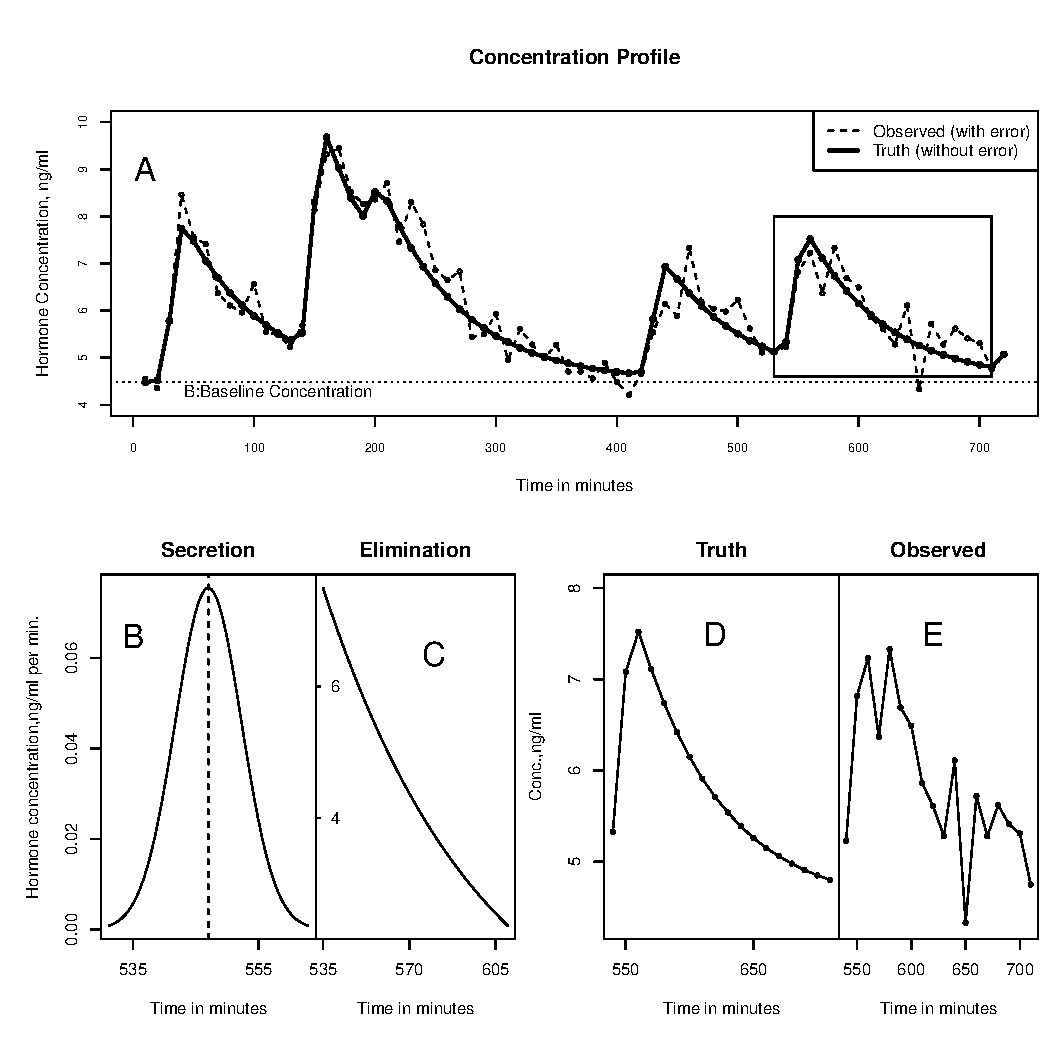
\includegraphics[width=5in]{deconvolution.pdf}
    \end{center}
   \caption{Graphic demonstration of the deconvolution model. 1A is a hormone concentration profile over time. The dashed line is the observed concentration and the black line is the truth from the computer simulation. The dotted line at the bottom is the non-pulse concentration, which is constant over the day in this application. The box shows a single pulse. The components of this pulse are shown in panel 1B to 1E. Graph 1B is the secretion of this pulse, assumed to have a normal shape in this simulation. Other shapes used include Weibull. The size of the pulse is the area under the curve (AUC). The pulse width is the standard deviation of the normal curve, and the center of the normal is the pulse location. The elimination is assumed to follow an exponential decay curve (Figure 1C).  Other more complex models are possible \cite{Keenan08}; however, with typical sampling protocols, estimating more complex elimination functions is not always practical \cite{Mauger95}. Figure 1D shows the true pulse shape combining 1B and 1C, and 1E shows the same pulse with observed error. The model error is assumed Gaussian as in standard regression approaches.
}
   \label{fig:deconv}
\end{figure}

\section{The secretion function, $S_i(z;\boldsymbol{\theta}_{s,i})$} It is common for pulsatile secretion to be defined by a series of Gaussian components, each with ``pulse specific" parameters. So, assuming subject $i$ experiences $N_i$ pulses by the end of the study,

\setstretch{1.0}

\begin{equation}
S_i(z,\boldsymbol{\theta}_{s,i}) = \sum_{k=1}^{N_i}  \frac{\alpha_{ik}}{\sqrt{2\pi\omega_{ik}}}e^{-\frac{1}{2\omega_{ik}}(z-\tau_{ik})^2}
\label{eq:Secretion}
\end{equation}

\setstretch{2.0}

The values $\alpha_{ik}$, $\omega_{ik}$, and $\tau_{ik}$ are the mass, width, and location, respectively, for the $k$th pulse. Therefore, $\boldsymbol{\theta}_{s,i} = (\boldsymbol{\alpha}_i,\boldsymbol{\omega}_i,\boldsymbol{\tau}_i)^T$, where $\boldsymbol{\alpha}_i$ represents the vector of pulse masses: $\boldsymbol{\alpha}_i = (\alpha_{i1},\alpha_{i2},...,\alpha_{iN_i})^T$ and $\boldsymbol{\omega}_i$ and $\boldsymbol{\tau}_i$ are defined as the vectors of pulse widths and pulse locations, respectively.
\setstretch{2.0}


We assume that the pulse specific parameters have the following distributions:

\setstretch{1.0}

$$
\log \alpha_{ik} \stackrel{iid}{\sim} N(\mu_{ai},\nu^2_{ai})
$$
$$
\log \omega_{ik} \stackrel{iid}{\sim} N(\mu_{wi}, \nu^2_{wi})
$$
$$
\tau_{ik}|N_i \stackrel{iid}{\sim} U^{(3N_i + 2)}[a,b]
$$

\setstretch{2.0}

\section{The elimination function, $E_i(t_j-z;\boldsymbol{\theta}_{e,i})$} It is common for elimination to be described by the exponential distribution with decay rate $\lambda_i$, or equivalently, half-life $H_i$.

\setstretch{1.0}

\begin{equation}
E_i(t_j-z,\boldsymbol{\theta}_{e,i}) =e^{-\lambda_i(t_j-z)} = e^{-\frac{\log 2}{H_i}(t_j-z)}
\label{eq:Elimination}
\end{equation}

\setstretch{2.0}

Therefore, $\boldsymbol{\theta}_{e,i} = H_i$.

\section{The deconvolution model} Putting together the secretion (\ref{eq:Secretion}) and elimination (\ref{eq:Elimination}) functions, the statistical model of observed hormone concentration at time $t_j$ is:

\setstretch{1.0}

\beq
\log[y_i(t_j)]=\log\left[B_i + \int_{-\infty}^{t_j} \sum_{k=1}^{N_i}  \frac{\alpha_{ik}}{\sqrt{2\pi\omega_{ik}}}e^{-\frac{1}{2\omega_{ik}}(z-\tau_{ik})^2} e^{-\lambda_i(t_j-z)}\,dz\right]+\epsilon_i(t_j)
\label{eq:DeconModel}
\eeq

\setstretch{2.0}

\noindent where $B_i$ is the time constant baseline concentration.\\
In summary, there are 8 common parameters for one subject: number of pulses ($n_i$), Baseline secretion ($B_i$), average pulse mass ($\mu_{ai}$), average pulse duration ($\mu_{wi}$), half-life ($H_i$), model error ($\epsilon_i$), variation between pulse mass ($\nu^2_{ai}$), and variation between pulse width ($\nu^2_{wi}$). The first 5 parameters usually have important physiological indications, while the last three variance parameters can be treated as nuisance parameters.  Estimation of each pulse is composed of 3 parameters: individual pulse mass ($\alpha_{ik}$), individual pulse duration ($\omega_{ik}$), and pulse location ($\lambda_{ik}$). A graphic demonstration of the deconvolution model is shown in Figure \ref{fig:deconv}.







\section{Implementation}








\chapter{BDMCMC:Single hormone-single subject modeling}
\section{General Usage Information}
Bayesian Analysis of Pulsatile Hormone Levels (BAPHL) is a software package developed by Nichole Carslon's research group to analyze pulsing hormones by a front end GUI interface in a Bayesian way. There are three sets of inputs need to be specified by user: 1) the input file, input and output directory,  and parameters that contain information about hormone time series observations for each subject, which is described in \ref{intro:general}; 2) the parameters in the prior distribution, which is described in \ref{intro:p1} to \ref{p2}; 3) the parameters in the MCMC implementations \ref{intro:mcmc}. BAPHL also provides default values for 2) and 3). The default values of the prior distribution is for vague prior information, which minimizes the influence of the prior and let the data dominates the estimation. The default values for the implementation parameters are set to achieve optimal MCMC performance. The output of BAPHL contains the conditional posterior distribution of each parameter for each subject, presented in both raw output of the MCMC (\ref{o1}) and graphic and tabular summarization (\ref{o2} and \ref{o3}. Section \ref{qs} demonstrates a brief introduction on how to implement BAPHL to analyze pulsatile hormones using default values for prior distribution and the MCMC implementation in the console.

\newpage
\section{Quick Start} \label{qs}


The software is started by executing the file RAPHL.exe.  The main window that looks like Figure \ref{startscreen} will appear.  This windows has a menu bar, a console output field, a panel of buttons to the right of the console output, and a progress bar on the bottom.
\begin{figure}
  \centering
  % Requires \usepackage{graphicx}
  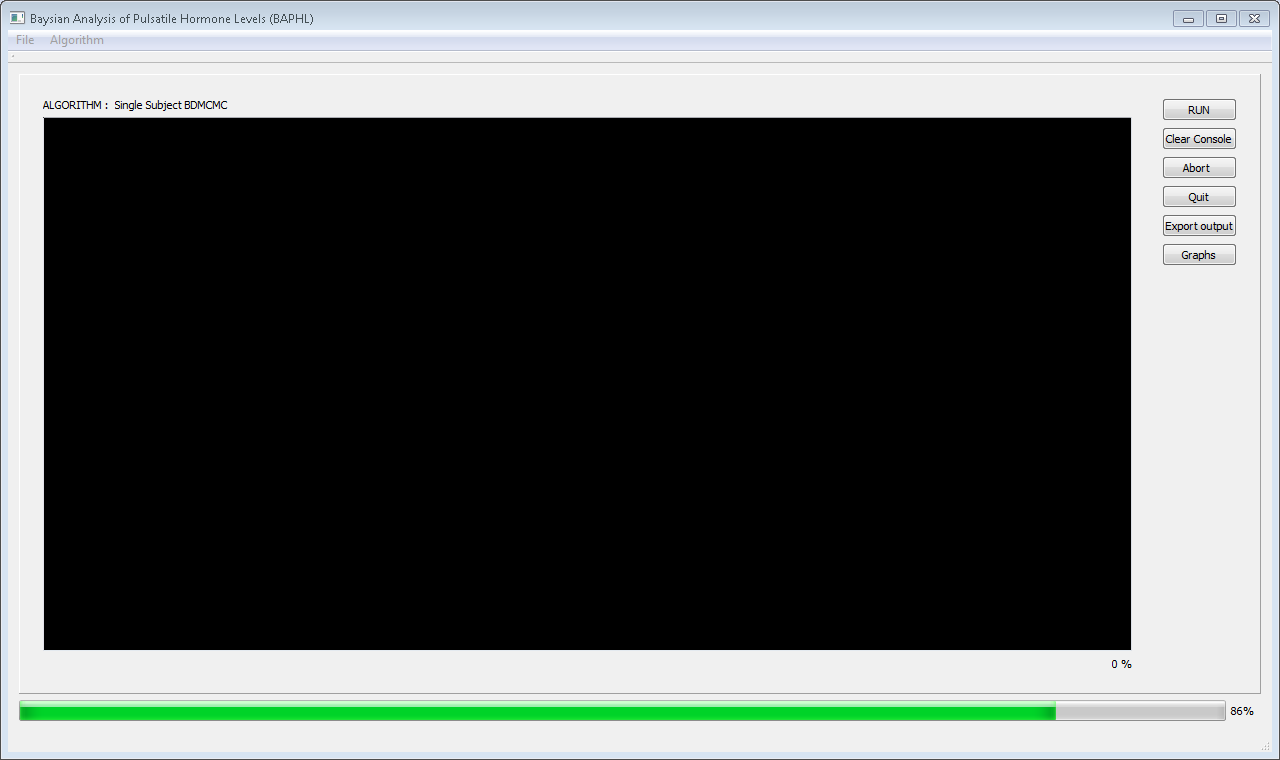
\includegraphics[width=\textwidth]{start.PNG}\\
  \caption{Start Screen of BAPHL}\label{startscreen}
\end{figure}
\newpage
To use the BAPHL software, the user
Start a new analysis by clicking the ``Algorithm'' menu item and then ``Single Subject''.  A dialog box as shown in Figure \ref{singlesubject} will pop up.\\
\begin{figure}
  \centering
  % Requires \usepackage{graphicx}
  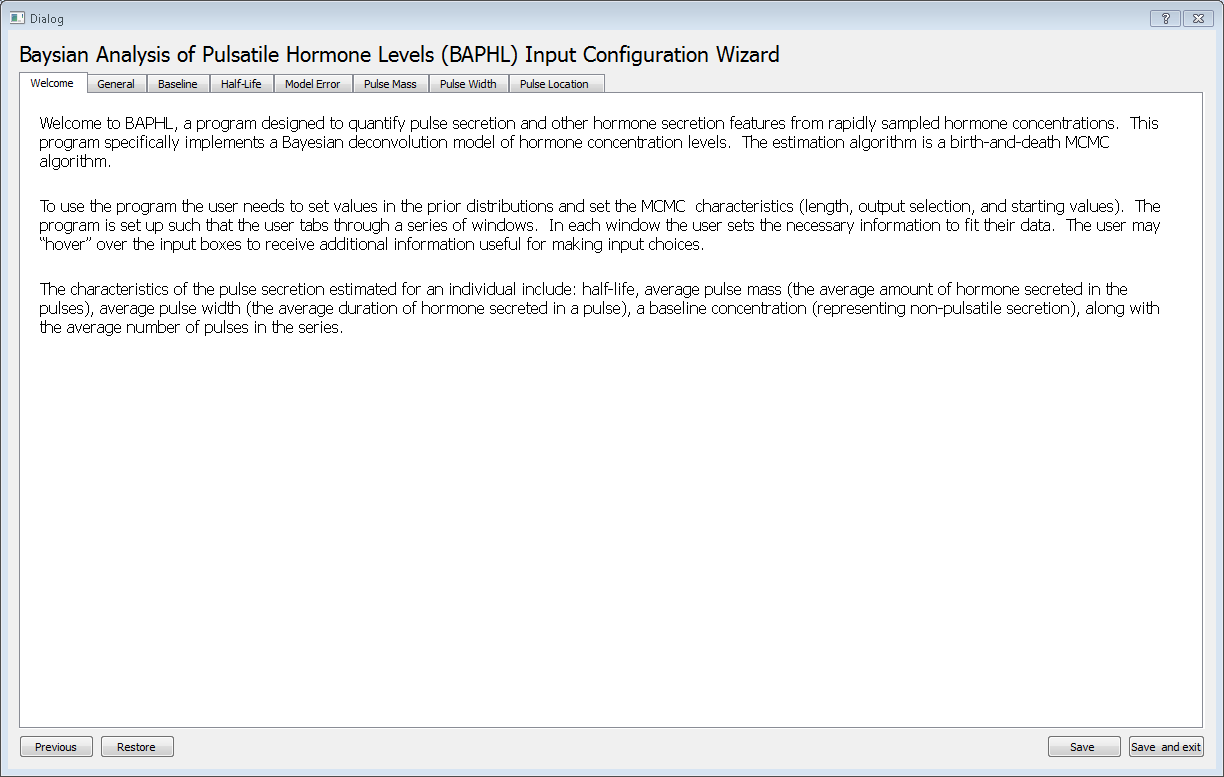
\includegraphics[width=\textwidth]{singlesubject.PNG}\\
  \caption{Bayesian Analysis of Pulsatile Hormone Levels (BAPHL) Input Configuration Wizard}\label{singlesubject}
\end{figure}

\newpage
Click the ``General'' tab (Figure \ref{general}) in the dialog box.  Click ``Browse'' to select the input data file, which defaults to an example file named ``subjmodel61s1.dat''.  Change ``Rate of writing to files (Iterations)" to 10, and ``Rate of console refresh (Iterations)'' to 50.  The two parameters specify how often data is output to files and the main screen.  Enter 10 for Constant birth rate.  Enter 1000 for MCMC Iteration Count. Enter 5000 for Burn in count (Iterations).\\
\begin{figure}
  \centering
  % Requires \usepackage{graphicx}
  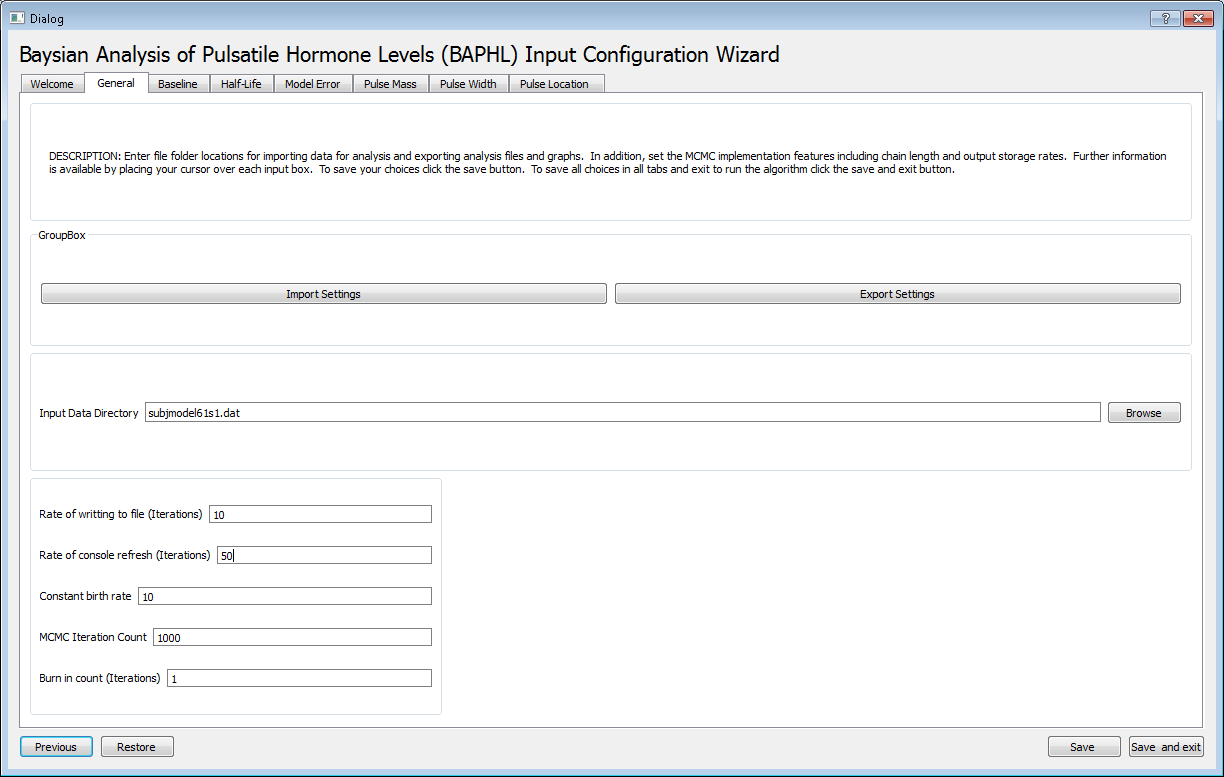
\includegraphics[width=\textwidth]{generaltab.PNG}\\
  \caption{"General" Tab}\label{general}
\end{figure}

\newpage
Click the ``Baseline'' tab (Figure \ref{baseline}). Enter 3 for Prior mean, 100 for Prior variance, 0.015 for Proposal variance, and 2.5 for Starting value.\\
\begin{figure}
  \centering
  % Requires \usepackage{graphicx}
  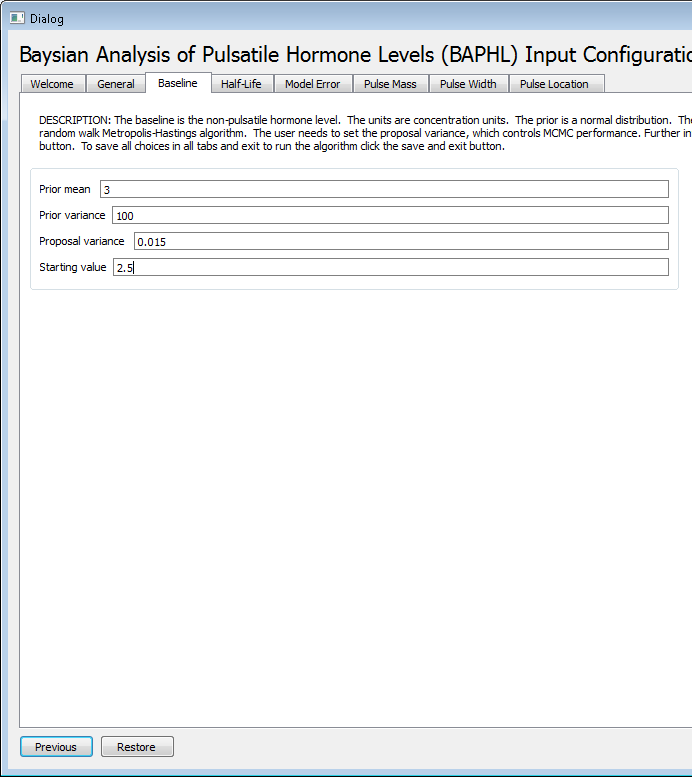
\includegraphics[width=\textwidth]{baselinetab.PNG}\\
  \caption{Baseline tab}\label{baseline}
\end{figure}
\newpage
Click the ``Half-Life'' tab (Figure \ref{halflife}). Enter 45 for Prior mean, 100 for Prior variance, 0.90 for Correlation proposal for halflife, 50 for Proposal variance, and 45 for Starting value.
\begin{figure}
  \centering
  % Requires \usepackage{graphicx}
  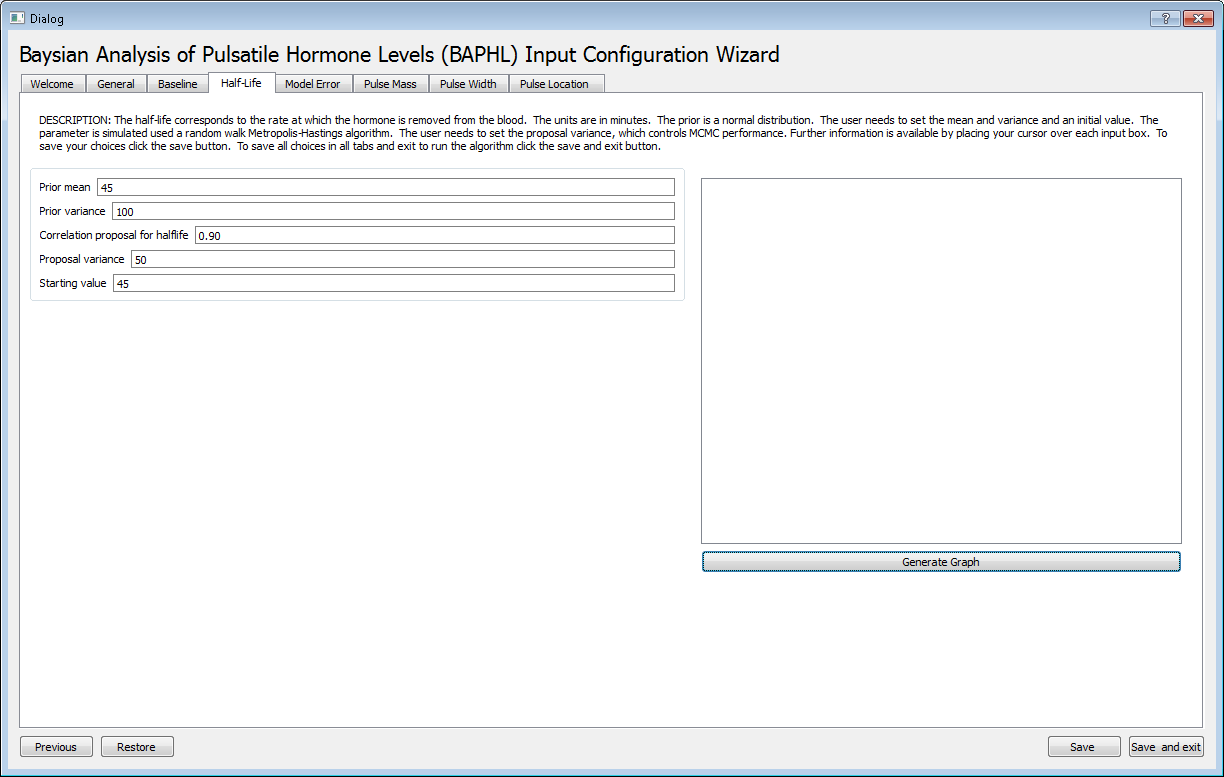
\includegraphics[width=\textwidth]{halflifetab.PNG}\\
  \caption{Half-Life tab}\label{halflife}
\end{figure}
\newpage
Click the ``Model Error'' tab (Figure \ref{modelerror}). Enter 0.0001 for Shape of Prior, 0.0001 for Rate of Prior, and 0.25 for Initial value for mode error.

\begin{figure}
  \centering
  % Requires \usepackage{graphicx}
  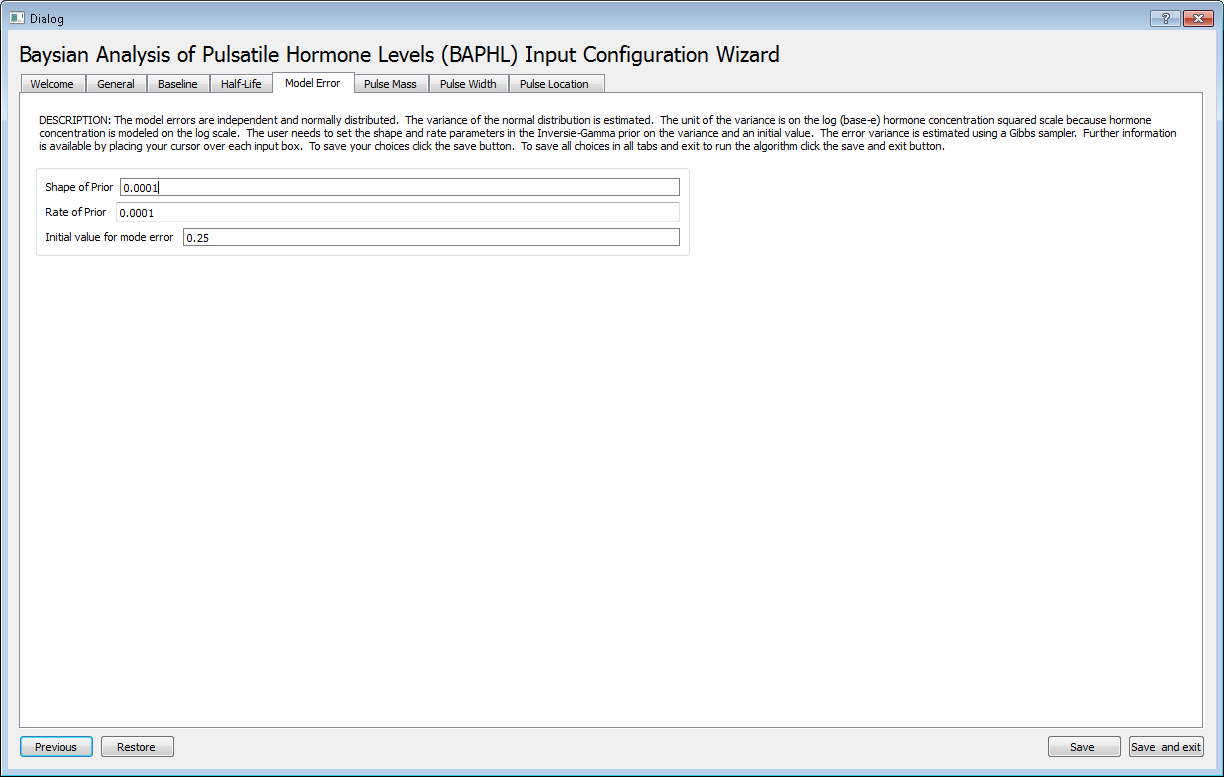
\includegraphics[width=\textwidth]{modelerrortab.PNG}\\
  \caption{Model Error tab}\label{modelerror}
\end{figure}
\newpage
Click the ``Pulse Mass'' tab (Figure \ref{pulsemass}). The pulse mass is modeled on the log-scale. Enter 1 for Mean of prior for mean pulse mass, 10 for variance of prior for mean pulse mass, 200 for Prior On SD of pulse masses, 0.9 for Proposal variance for individual pulse masses, 0.5 for Proposal variance for SD of pulse masses, 1 for Initial value for mean pulse mass, and 1 for Initial value SD of pulse masses.

\begin{figure}
  \centering
  % Requires \usepackage{graphicx}
  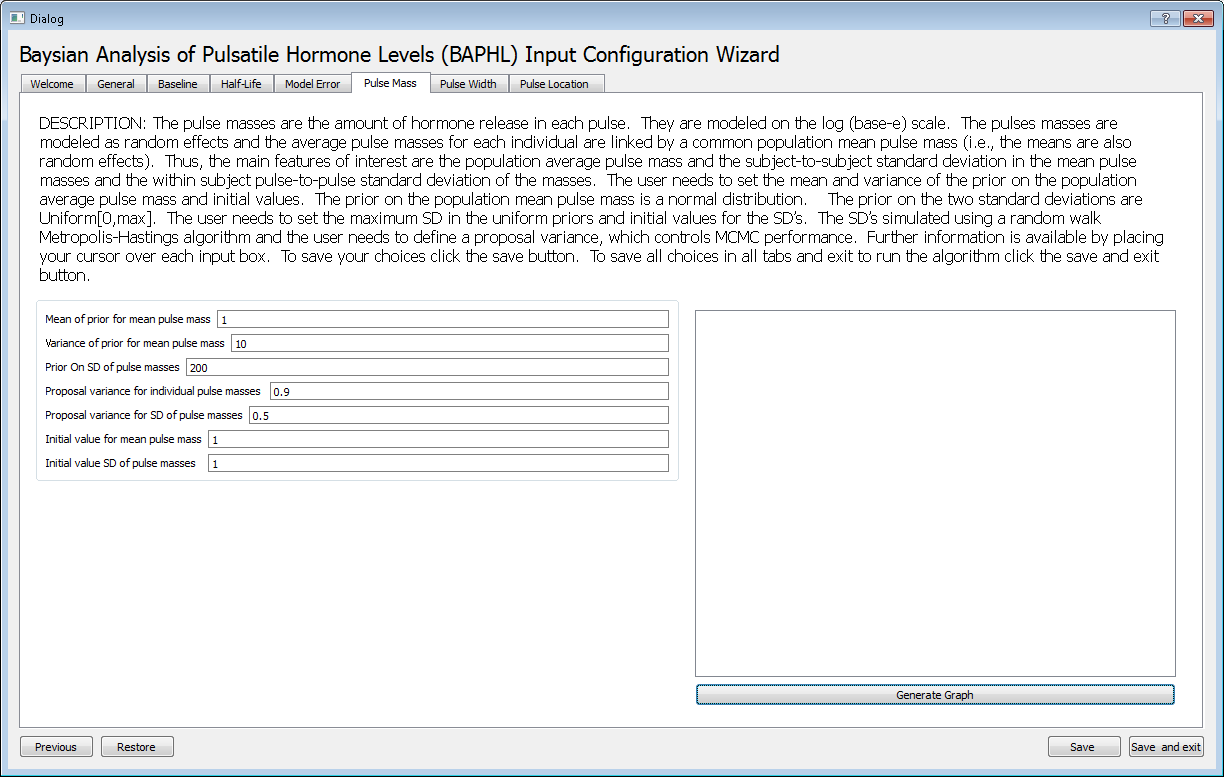
\includegraphics[width=\textwidth]{pulsemasstab.PNG}\\
  \caption{Model Error tab}\label{pulsemass}
\end{figure}
\newpage
Click the ``Pulse Width'' tab (Figure \ref{pulsewidth}). The pulse mass is modeled on the log-scale. Enter 1.5 for Mean of prior for mean pulse width, 10 for Variance of prior for mean pulse width, 200 for Prior on SD of pulse widths, 4 for Proposal variance for individual pulse widths, 6 for Proposal variance for SD of pulse widths, 1 for Initial value SD of pulse width, and 1.5 for Initial value of mean pulse width.

\begin{figure}
  \centering
  % Requires \usepackage{graphicx}
  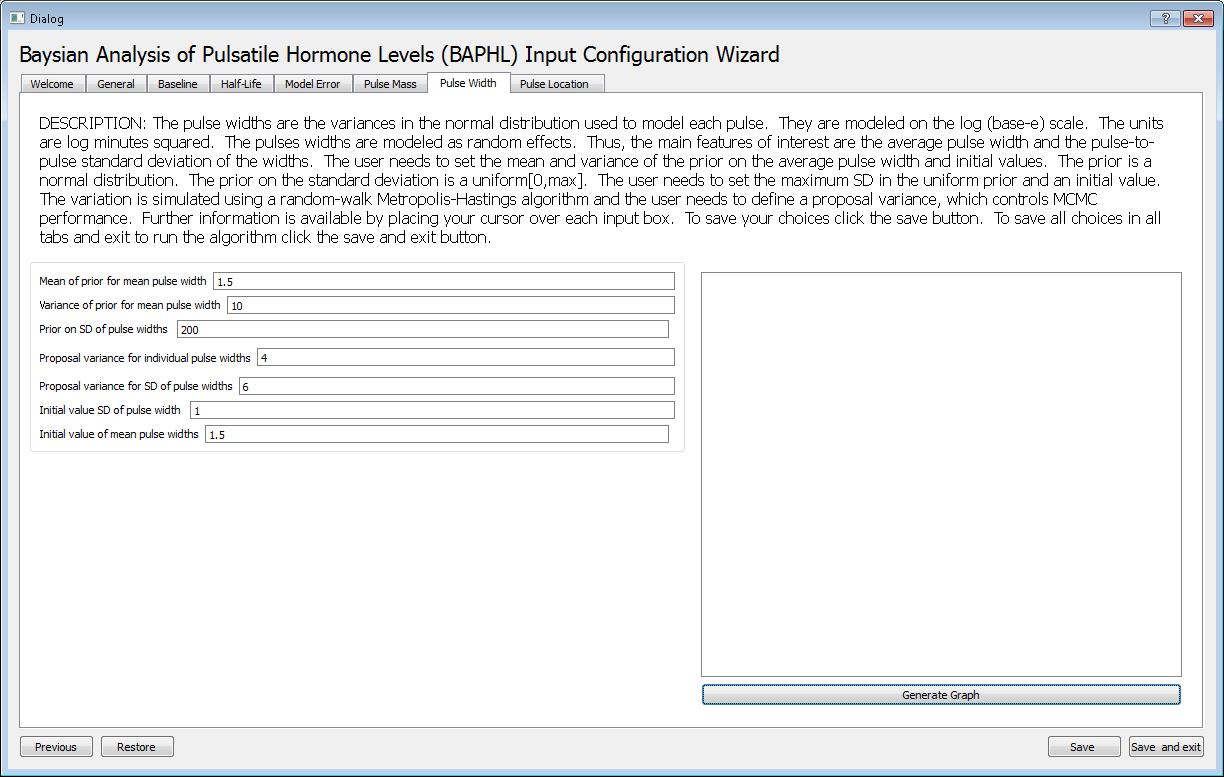
\includegraphics[width=\textwidth]{pulsewidthtab.PNG}\\
  \caption{Pulse Width tab}\label{pulsewidth}
\end{figure}
\newpage
Click the ``Pulse Location'' tab (Figure \ref{pulselocation}). Enter 12 for Rate in poisson prior on number of pulses in a series, 3 for Pulse Location Distn Order Stat, 1 for Proposal variance for individual pulse location, and 1 for Length of birth-death process for each iteration.

\begin{figure}
  \centering
  % Requires \usepackage{graphicx}
  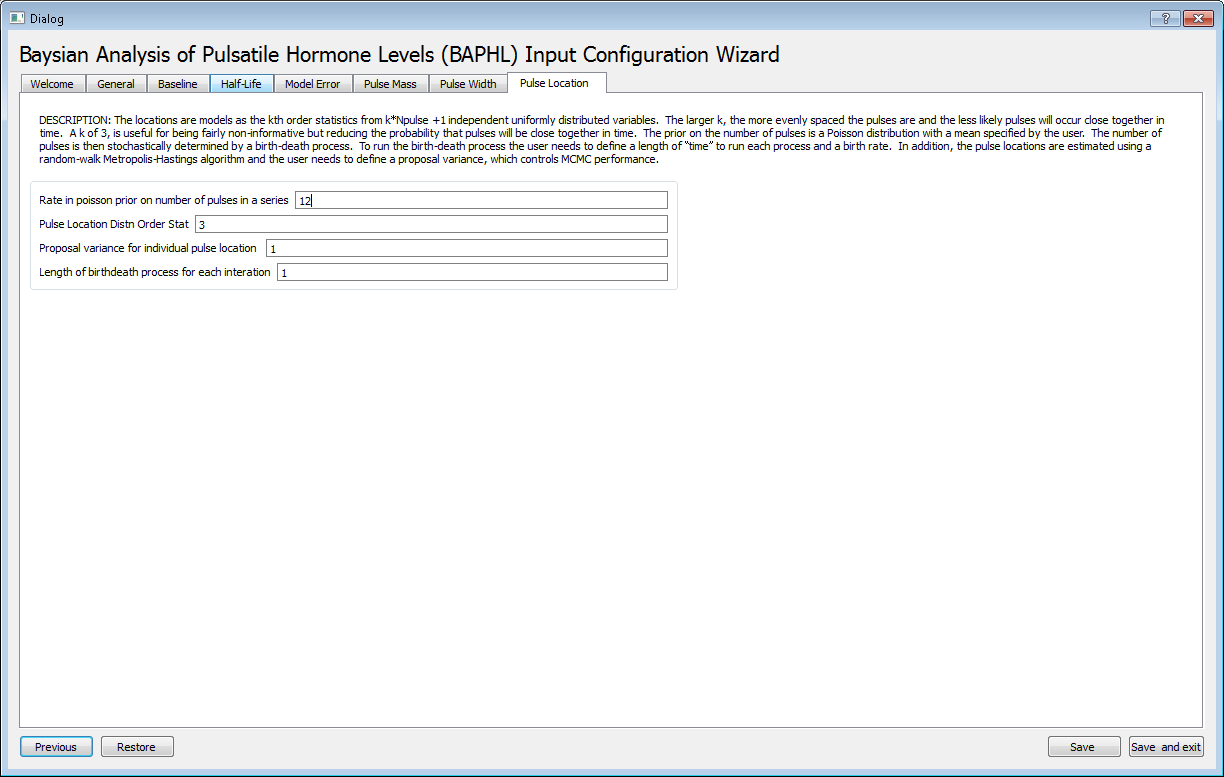
\includegraphics[width=\textwidth]{pulselocationtab.PNG}\\
  \caption{Pulse Location tab}\label{pulselocation}
\end{figure}
\newpage
Click on ``Save'' button to save the settings in this dialog box.  Activate the main window by clicking on the window title.  Click on the ``Run'' button to start the analysis.  The console output field will be populated by the results of every 50 iteration, as specified in ``General'' tab (Figure \ref{general}).
\begin{figure}
  \centering
  % Requires \usepackage{graphicx}
  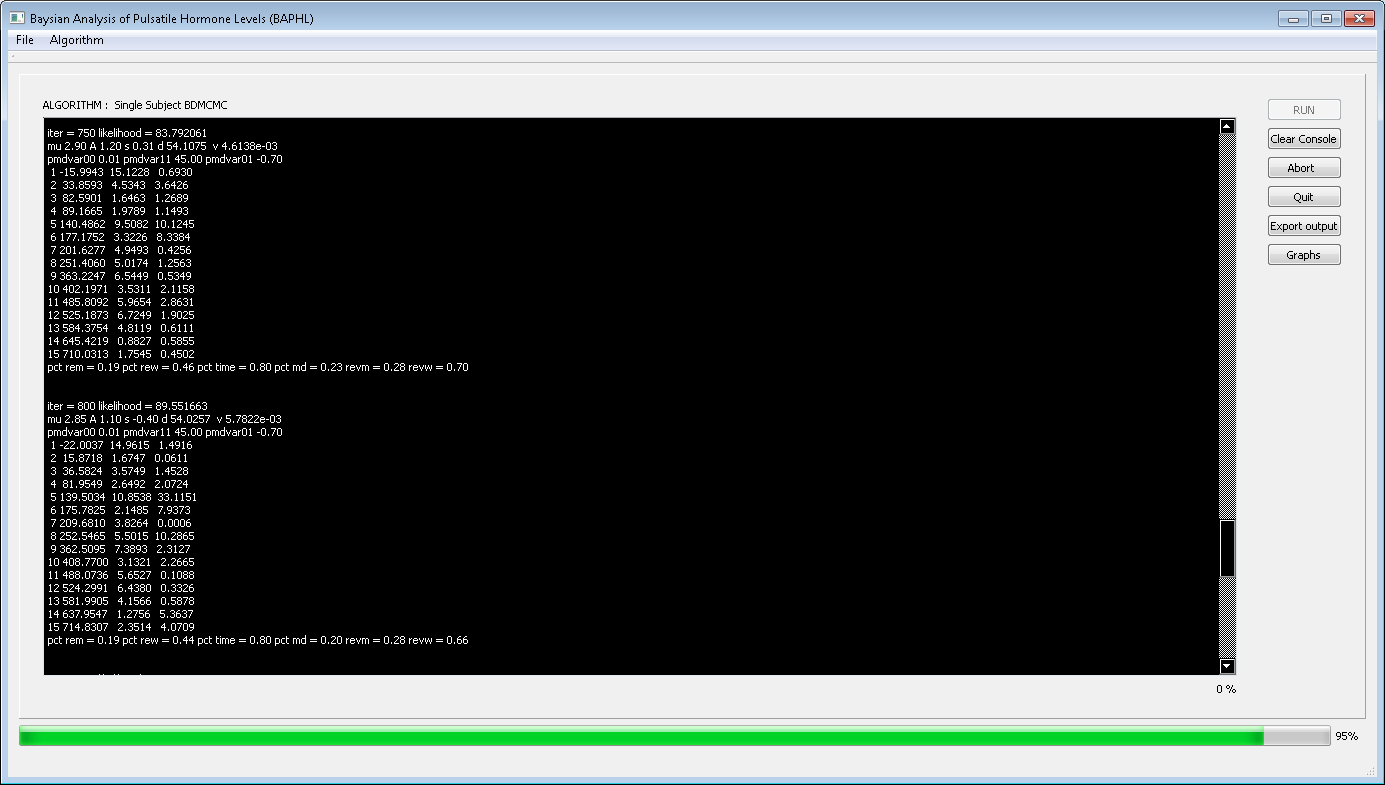
\includegraphics[width=\textwidth]{consoleoutput.PNG}\\
  \caption{Console output}\label{consoleoutput}
\end{figure}

After console stops refreshing,the output can be demonstrated by clicking the ``Graphs'' tab and the output can be exported and saved in  a directory by clicking the ``Export output'' tab.

\section{Data File Formats}\label{intro:general}
In each of the input files that contains the time series for observation hormone data, the first row will be ignored by the software.
The first column is the index of observations and will be ignored by the software. The second column is the time of observation, and the third column is the measured concentration at each time point. User does not need to specify the inter-assay or intra-assay correlation coefficients. The length of each column needs to be the same.  Missing observations, if present, should be estimated by interpolating between neighboring observations.
\section{Graphing the Data}
A graphing tool is utilized to demonstrate the  prior distribution visually for each parameter. By clicking on the ``Generate Graph'' button, the curve of the probability density function (PDF) of the prior normal distribution will be generated. A normal distribution is usually bell-shaped and symmetric. The peak (mode) of the distribution represents most likely values \emph{a priori} and the range of X-axis should cover the range of all biological possible values of the parameter.
\section{General Tab}\label{intro:mcmc}
To use the BAPHL software, the user needs to provide the MCMC parameters, including how many iteration to run, the frequency of writing to file and console refresh, burn-in count, and birth-rate in the birth-death process. The default value for MCMC number of iterations is 500,000.  The number of iterations needed to achieve good mixing properties and to collect enough information to summarize the feature of each parameters ranges from ranges from 150,000 to 1,000,000. The rate of writing to file specify how often the program output the current value of the parameter in the MCMC simulation, and the default value is one output every 50 iteration. This process is called thinning, and it is useful to reduce demands for data storage and lower the correlation between successive draws, and therefore enhance the performance of the MCMC simulation. However, with increasing spacing between saving values, the numbers of iteration required to collect the information of the posterior distribution is also increased. The suggested value for thinning is from 20 to 100 iterations. The rate of console refresh specifies how often the output is written to screen, and the default value is every 5000 iterations. The screen output contains the current values of parameters, including the subject-level, such as baseline secretion, half-life and average pulse mass; and  pulse-specific parameters for each secretion event, including pulse mass, pulse width the pulse location, together with acceptance rate of each parameter if drawn using Metropolis-Hasting algorithm. Good MCMC behavior is more likely when the acceptance rate is between 25\% to 50\%.  Larger accepted rate can be achieved by decreasing proposal variance, and vice versa.  Burn-in count is the number of the MCMC draws at the beginning that will be discarded when summarizing the posterior distribution. Usually the first 5\% to 25\% of the MCMC draws are discarded to lower the dependence of the posterior distribution on starting values. The birth-rate is set as the possible number of pulses in each subject. For human luteinizing hormone (LH), the pulsing frequency is usually 1 pulse per hour. Deviation from correct birth-rate is not likely to result in biased estimation, but will cause longer time to the MCMC to converge.


\section{Baseline Tab}\label{intro:p1}
The Baseline is the non-pulsatile, constant hormone level. The prior is a normal distribution with user-specified mean and variance. We suggest to set the mean equal to the fitted value from other sources, e.g., 4 concentration units for  human LH, and a relatively larger,or uninformative variance, like 1000. The posterior distribution of the parameter is simulated using a random walk Metropolis-Hastings algorithm. The user needs to specify the starting value and the proposal variance which controls MCMC performance. A starting value is usually set equal or closed to the prior mean, and the posterior distribution should not depend on the starting value if the MCMC is mixing well.  A proposal variance is used to draw each MCMC simulation. The suggested proposal variance for baseline is 0.015 to start with,and is updated every 500 iterations in the first 2000 iterations. The proposal variance governs the performance of the MCMC simulation, and should be properly chosen so that the acceptance rate is between 25\% to 50\%. If the acceptance rate is below 25\%, the user is suggested to use a smaller proposal variance and vice versa.
\section{Half-life Tab}
The half-life corresponds to the rate at which the hormone is removed from the blood. More specifically, the half-life is the amount of time required for the hormone concentration to fall to half of its peak value. The prior is a normal distribution with user-specified mean and variance. We suggest to set the mean equal to the fitted value from other sources, e.g., 45 minutes for  human LH, and a relatively larger,or uninformative variance, like 1000. The posterior distribution of the parameter is simulated using a random walk Metropolis-Hastings algorithm. The user needs to specify the starting value, the proposal variance and correlation which controls MCMC performance. A starting value is usually set equal or closed to the prior mean, and the posterior distribution should not depend on the starting value if the MCMC is mixing well. A proposal variance is used to draw each MCMC simulation The suggested proposal variance for half-life is 50 to start with,and is updated every 500 iterations in the first 2000 iterations. The proposal variance governs the performance of the MCMC simulation, and should be properly chosen so that the acceptance rate is between 25\% to 50\%. If the acceptance rate is below 25\%, the user is suggested to use a smaller proposal variance and vice versa. The estimation of half-life is highly negatively correlated with baseline, and they are drawn simultaneously in each MCMC iteration. A correlation proposal for baseline and half-life also needs to be specified, and the default value is -0.85.
\section{Model Error Tab}
The model error are independent and normally distributed with mean 0. The unit of log is on the log (base-e) unit because the hormone concentration needs to be positive and is modeled on the log scale. A conjugate gamma family prior is used for model error and the posterior is drawn using a Gibbs sampler. The user needs to specify the rate and shape parameter for the inverse-Gamma distribution, which are both 0.0001 by default (here is an error: the default is 0.01 in hover). Values closed to 0 imply a uninformative prior for both rate and shape.
\section{Pulse Mass Tab}
The pulse masses are the amount of hormone released in each pulse. They are modeled using a random effect model on the log scale, with a unique mean and variance for each subject in the single subject model, and average pulse masses for each subjected linked by a common population mean pulse mass in the population. Thus, the main features of interest are the average pulse mass and pulse-to-pulse variability in one subject in the single subject model, and population-average pulse mass with subject-to-subject variability in the population model. The prior for pulse mass mean is a normal distribution, and the prior for pulse mass variance is a uniform distribution of [0, Max]. In the single-subject model, the user needs to specify the mean and variance for the normal prior distribution, and the Max for the uniform distribution. We suggest to set the mean equal to the fitted value from other sources, e.g., 1 (on the log scale) for human LH, and a relatively large value for the prior variance (the default is 1000). We also suggest using a larger upper boundary for the variance, and the default value is 200. A Gibbs sampler is utilized to estimate the mean pulse mass, and the user only needs to specify the initial value for mean pulse mass.  A starting value is usually set equal or closed to the prior mean, and the posterior distribution should not depend on the starting value if the MCMC is mixing well. The individual pulse mass and pulse mass variance and simulated using Metropolis-Hastings algorithm. A proposal variance is used to draw each MCMC simulation. The suggested proposal variance  is 0.9 for individual pulse mass and 0.5 for pulse mass variance to start with,and is updated every 500 iterations in the first 2000 iterations. The proposal variance governs the performance of the MCMC simulation, and should be properly chosen so that the acceptance rate is between 25\% to 50\%. If the acceptance rate is below 25\%, the user is suggested to use a smaller proposal variance and vice versa.

\section{Pulse Width Tab}
The pulse width describes the spread, or duration of each pulsing event. They are modeled using a random effect model on the log scale, with a unique mean and variance for each subject in the single subject model, and average pulse width for each subjected linked by a common population mean pulse mass in the population. Thus, the main features of interest are the average pulse width and pulse-to-pulse variability in one subject in the single subject model, and population-average pulse width with subject-to-subject variability in the population model. The prior for pulse width mean is a normal distribution, and the prior for pulse width variance is a uniform distribution of [0, Max]. In the single-subject model, the user needs to specify the mean and variance for the normal prior distribution, and the Max for the uniform distribution. We suggest to set the mean equal to the fitted value from other sources, e.g., 1 (on the log scale) for human LH, and a relatively large value for the prior variance (the default is 1000). We also suggest using a larger upper boundary for the variance, and the default value is 200. A Gibbs sampler is utilized to estimate the mean pulse width, and the user only needs to specify the initial value for mean pulse width.  A starting value is usually set equal or closed to the prior mean, and the posterior distribution should not depend on the starting value if the MCMC is mixing well. The individual pulse width and pulse width variance and simulated using Metropolis-Hastings algorithm. A proposal variance is used to draw each MCMC simulation. The suggested proposal variance  is 0.9 for individual pulse width and 0.5 for pulse width variance to start with,and is updated every 500 iterations in the first 2000 iterations. The proposal variance governs the performance of the MCMC simulation, and should be properly chosen so that the acceptance rate is between 25\% to 50\%. If the acceptance rate is below 25\%, the user is suggested to use a smaller proposal variance and vice versa.

\section{Pulse Locations Tab} \label{p2}
The locations are modeled as the $kth$ order statistics from $kN+1$ independent uniformly distributed random variable from a time window slightly larger than the observation time period, where $k$ is a user-specified integers, and N is the number of pulsing event. A larger $k$ yield more evenly spaced pulsed and thus less likely pulses that are too closed together. The default value for k is 3, which is fairly non-informative but reducing the probability that the pulses will be close together in time. The prior on the number of pulses is a Poisson distribution with a mean specified by the user. For human LH we suggest that the Poisson rate is 1 times the observation time in hours. The number of pulses is then stochastically determined by a birth-death process. The user needs to define the length of "time" to run each process, and the default value is 1. A larger value will facilitate pulse-fitting but takes longer time for each iteration. In addition, each pulse location is estimated using a random-walk Metropolis-Hastings algorithm and the user needs to define a proposal variance, which control MCMC performance. The suggested proposal variance  is 1 for pule location,and is updated every 500 iterations in the first 2000 iterations. The proposal variance governs the performance of the MCMC simulation, and should be properly chosen so that the acceptance rate is between 25\% to 50\%. If the acceptance rate is below 25\%, the user is suggested to use a smaller proposal variance and vice versa.

\newpage
\section{Console Output}\label{o1}
Once the estimation has started, The console output field will be populated by the results of every 50 iteration, as specified in ``General" tab (Figure \ref{console}). The Console output is very important in monitoring the performance of the MCMC simulation. The output includes all parameters of each pulses in the current iteration. The first column is the pulse order, the second column is the pulse mass, and the third column is the pulse width. It also includes the acceptance rate for each parameter if estimated using the Metropolis-Hastings algorithm ( Do we need to change the name shown in the console or I made a table for each output with a parameter?, like "pct md is the acceptance rate for pulse half-life and baseline).

\begin{figure}
  \centering
  % Requires \usepackage{graphicx}
  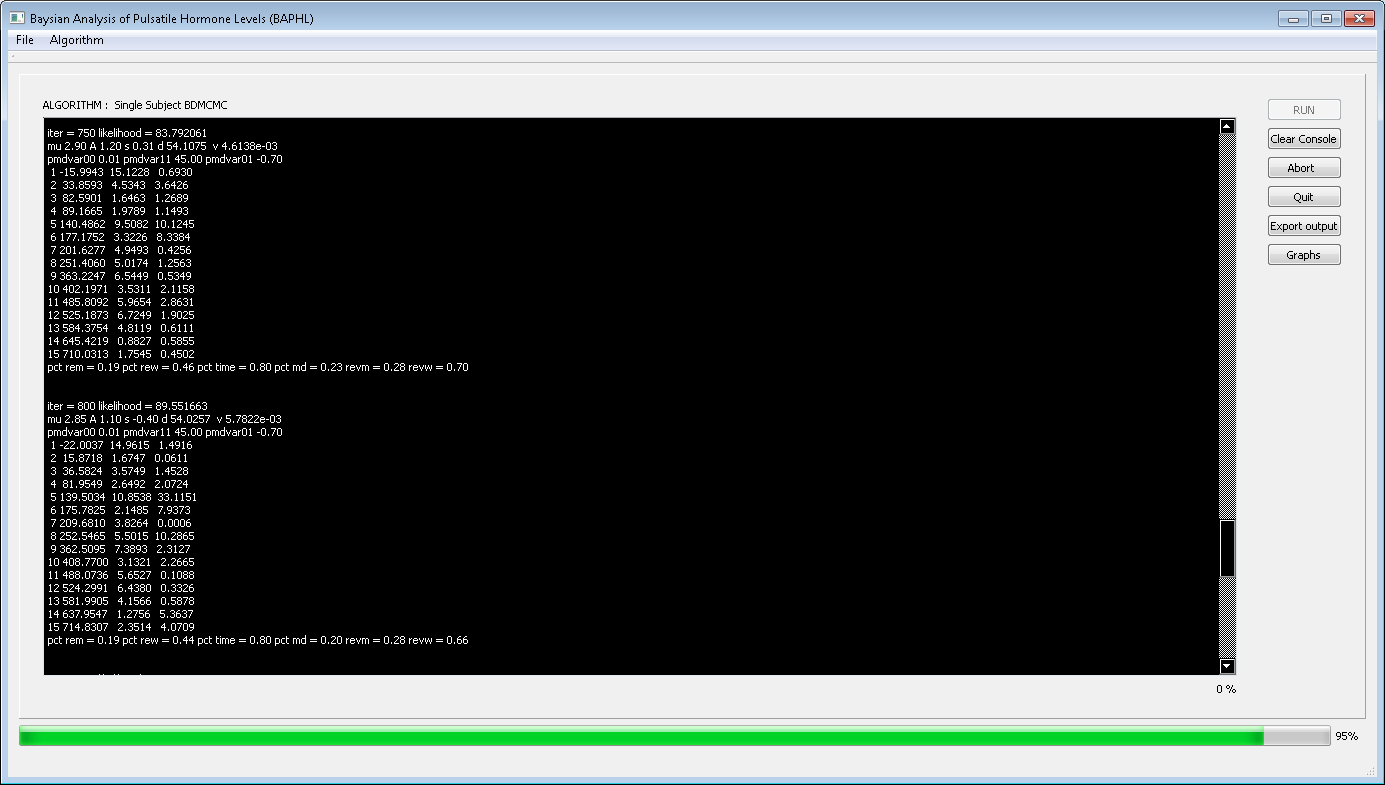
\includegraphics[width=\textwidth]{consoleoutput.PNG}\\
  \caption{Console Output tab}\label{console}
\end{figure}

\newpage
\section{Graphical Output} \label{o2}
After console stops refreshing,the output can be demonstrated by clicking the ``Graphs"  and the clicking the ``Generate Graph" tab  (Figure \ref{graph}). The left panel is set of graphs and right panel is the tabular summarization. Graph 1 to Graph 5 tab demonstrates the trace-plot for conditional posterior distribution in each iteration (left-hand side) and histogram of conditional posterior distribution for each parameter. The trace-plot are generated to conduct convergence diagnosis. A longer time to convergence is indicated When a chain takes longer time to move around the parameter space, and a modification in the proposal variance is needed to attain better MCMC mixing behavior.

\begin{figure}
  \centering
  % Requires \usepackage{graphicx}
  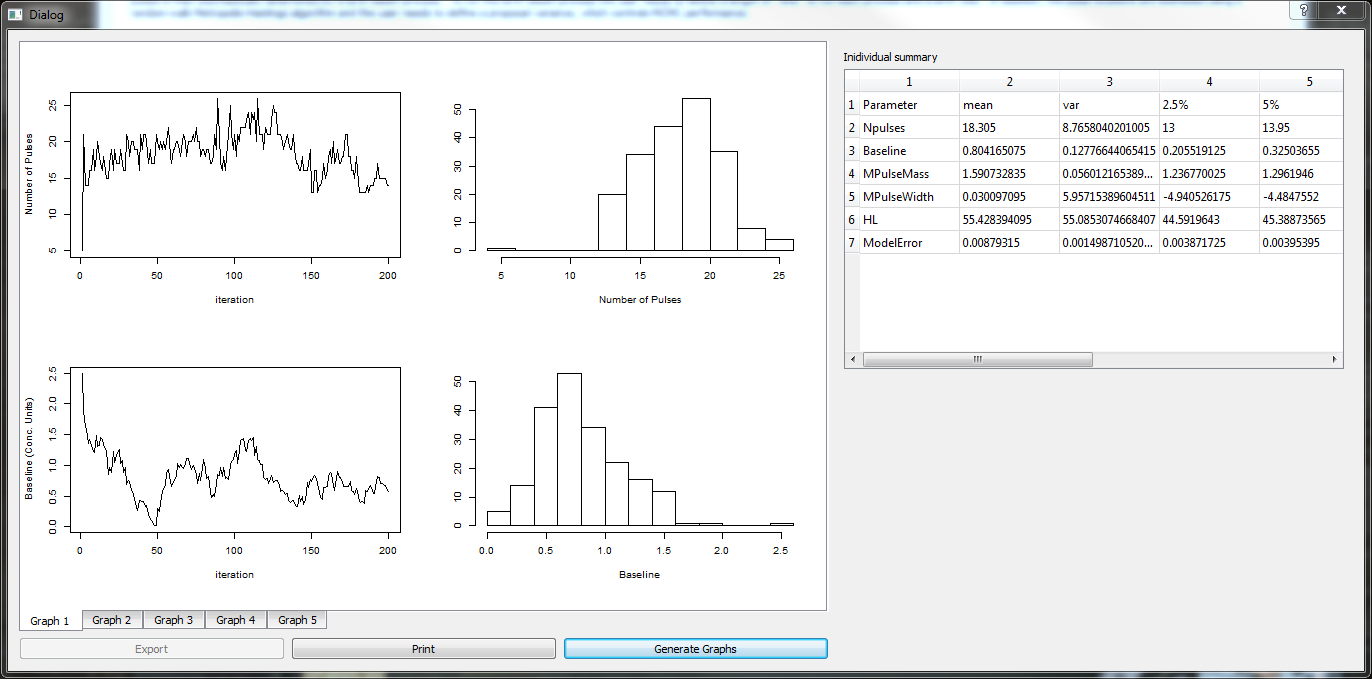
\includegraphics[width=\textwidth]{grapho.PNG}\\
  \caption{Graph Output tab}\label{graph}
\end{figure}



\section{Tabular Output} \label{o3}
The tabular output presents some summary statistics for each of the parameter on the subject level. More specifically, it gives mean, variance, 2.5\%, 5\%, 30\%, 95\% and 97.5\% quantiles calculated from the posterior distribution draws for count of pulses (2nd row),  baseline (3rd row), average pulse mass (log-scale, 4th row), average pulse width (log-scale, 5th row), half-life (6th row) and model error (7th row).

\chapter{Bayesian Modeling}
\section{Introduction of Bayesian Statistics}
The BAPHL estimates the pulse parameters under the Bayesian framework. The most important feature of Bayesian statistics is incorporating subjective knowledge and the confidence of that knowledge, quantified in the form of prior distribution, into interpretation of probabilities. In other words,
Bayesian analysis approach makes guesses about the values of the pulse characteristics (masses, widths, number, half-life, etc.) prior to observing any data and then reweights these guesses with knowledge from the observed data. The \emph{a priori} guesses about the values of the pulse features are called priors and are specified by the user. he data reweighted values of the pulse characteristics are called posteriors. The posterior represents the set of values of the pulse characteristic that are likely given the observed data and the prior.  To summarize Bayesian analysis, the mean of the posterior and its standard deviation or a credible interval are reported.  These can be conceptually linked (sort of) to the estimate and confidence interval in non-Bayesian approaches.
The frequentist assumes that a parameter is an unknown constant, and the inference made upon that parameter is presented in a point estimation and a corresponding variance related to the uncertainty. On the other way, a Bayesian considers a parameter as a random variable, and the estimation of the parameter is in the form of a posterior distribution.\\
The Bayes theorem, in its most common form, is
\setstretch{2.0}


\beq
P(\theta|X)=\frac{P(X|\theta)P(\theta)}{P(\theta)} = \frac{P(X|\theta)P(\theta)}{\sum_\theta P(X|\theta)P(\theta)}
\eeq

\setstretch{2.0}
$P(\theta)$ is the prior distribution of the parameter, $P(\theta|X)$ is the posterior distribution of the parameter of interest, and  $P(X|\theta)$ is the likelihood function of data given the parameter. The prior distribution is pre-specified before collecting data.The priors can be non-informative or informative .  When little is known about the hormone under study, the goal is to limit the influence of the prior to minimum (i.e., to be non-informative) and let the data dominate the estimation.  This is done by setting a large variance in the prior, reflecting lack of information available about the parameter.  When historical or biologic knowledge exists, we can incorporate that knowledge into the model by setting the mean of the prior to match prior information and setting a smaller variance.
\section{The Priors in the BAPHL.} \label{priors}
With one exception (pulse number), the priors distributions investigated in our analysis were normal distributions. The user defines the mean and the variance of each prior. The mean reflects historical knowledge regarding the value of the characteristic and the variance controls the confidence the user has about the mean. The priors can be informative (larger variance) or vague (smaller variance).
\section{Bayesian Estimation}

The posterior distribution of the parameter usually does not have a closed form  when the model have more than one parameters, as in the hormone concentrations. As a consequence, the desired distribution cannot be computed directly. Instead, they need to be simulated using Monte-Carlo Markov Chain (MCMC).In addition, the number of parameters is not fixed from iteration to iteration because the number of pulses is not known and also needs to be simulated. We consider using birth-death MCMC (BDMCMC) given its success in other pulse estimation problems . A single iteration of BDMCMC occurs in two stages. First, the number of components is simulated using a birth-death process. Next, conditional on the number of components, the remaining parameters are updated using traditional MCMC. The full algorithm iterates between these two steps.
In more detail, one iteration of our BDMCMC algorithm occurs as follows:

\noindent (1) Conditioned on the current values of ($\boldsymbol{\alpha}_i$, $\boldsymbol{\omega}_i$, $\boldsymbol{\tau}_i$, $\mu_{ai}$, $\mu_{wi}$, $\nu_{ai}$, $\nu_{wi}$, $B_i$, $H_i$, $N_i$, $\sigma_{\epsilon i}^2$), update $N_i$, $\boldsymbol{\alpha}_i$, $\boldsymbol{\omega}_i$, and $\boldsymbol{\tau}_i$ by running the birth-death process.

\noindent (2) Conditioned on the current values of ($\nu_{ai}$, $\nu_{wi}$, $B_i$, $H_i$, $N_i$, $\boldsymbol{\alpha}_i$, $\boldsymbol{\omega}_i$, $\boldsymbol{\tau}_i$, $\sigma_{\epsilon i}^2$), update $\mu_{ai}$ and $\mu_{wi}$, each by Gibbs sampler \cite{Geman}.

\noindent (3) Conditioned on the current values of ($\mu_{ai}$, $\mu_{wi}$, $B_i$, $H_i$, $N_i$, $\boldsymbol{\alpha}_i$, $\boldsymbol{\omega}_i$, $\boldsymbol{\tau}_i$, $\sigma_{\epsilon i}^2$), update $\nu_{ai}$ and $\nu_{wi}$, each by a random walk Metropolis-Hastings sampler.

\noindent (4) Conditioned on the current values of ($\mu_{ai}$, $\mu_{wi}$, $\nu_{ai}$, $\nu_{wi}$, $N_i$, $\boldsymbol{\alpha}_i$, $\boldsymbol{\omega}_i$, $\boldsymbol{\tau}_i$, $\sigma_{\epsilon i}^2$), update $B_i$ and $H_i$ by a Metropolis-Hastings sampler. These are drawn together since their estimates are highly correlated.

\noindent (5) Conditioned on the current values of ($\mu_{ai}$, $\mu_{wi}$, $\nu_{ai}$, $\nu_{wi}$, $N_i$, $B_i$, $H_i$, $\boldsymbol{\tau}_i$, $\sigma_{\epsilon i}^2$), update $(\alpha_{i1}, \omega_{i1}, \alpha_{i2}, \omega_{i2}, ... ,\alpha_{iN_i}, \omega_{iN_i})$, each by a Metropolis-Hastings sampler.

\noindent (6) Conditioned on the current values of ($\mu_{ai}$, $\mu_{wi}$, $\nu_{ai}$, $\nu_{wi}$, $N_i$, $B_i$, $H_i$, $\boldsymbol{\alpha}_i$, $\boldsymbol{\omega}_i$, $\sigma_{\epsilon i}^2$), update $(\tau_{i1},\tau_{i2},...,\tau_{iN_i})$, each by a Metropolis-Hastings sampler.

\noindent (7) Conditioned on the current values of ($\mu_{ai}$, $\mu_{wi}$, $\nu_{ai}$, $\nu_{wi}$, $N_i$, $B_i$, $H_i$, $\boldsymbol{\alpha}_i$, $\boldsymbol{\omega}_i$, $\boldsymbol{\tau}_i$), update $\sigma_{\epsilon i}^2$ by Gibbs sampler.

\noindent (8) Return to step (1).



\bibliographystyle{ama}
\bibliography{ref}


\end{document}
